\documentclass[border=20pt, tikz]{standalone}
\usepackage{tikz}
\usepackage{amsmath,amssymb}
\usetikzlibrary{positioning, arrows.meta, fit, backgrounds, calc, shapes.geometric, decorations.pathreplacing}

% ==============================================================================
%  HYALINE V2-D: READOUT & CLASSIFICATION HEAD DETAIL
% ==============================================================================

% --- Colors ---
\definecolor{egnnCol}{HTML}{533483}
\definecolor{jkCol}{HTML}{7b68ee}
\definecolor{globalCol}{HTML}{9370db}
\definecolor{concatCol}{HTML}{ba55d3}
\definecolor{mlpCol}{HTML}{4169e1}
\definecolor{outputCol}{HTML}{e94560}

\begin{document}
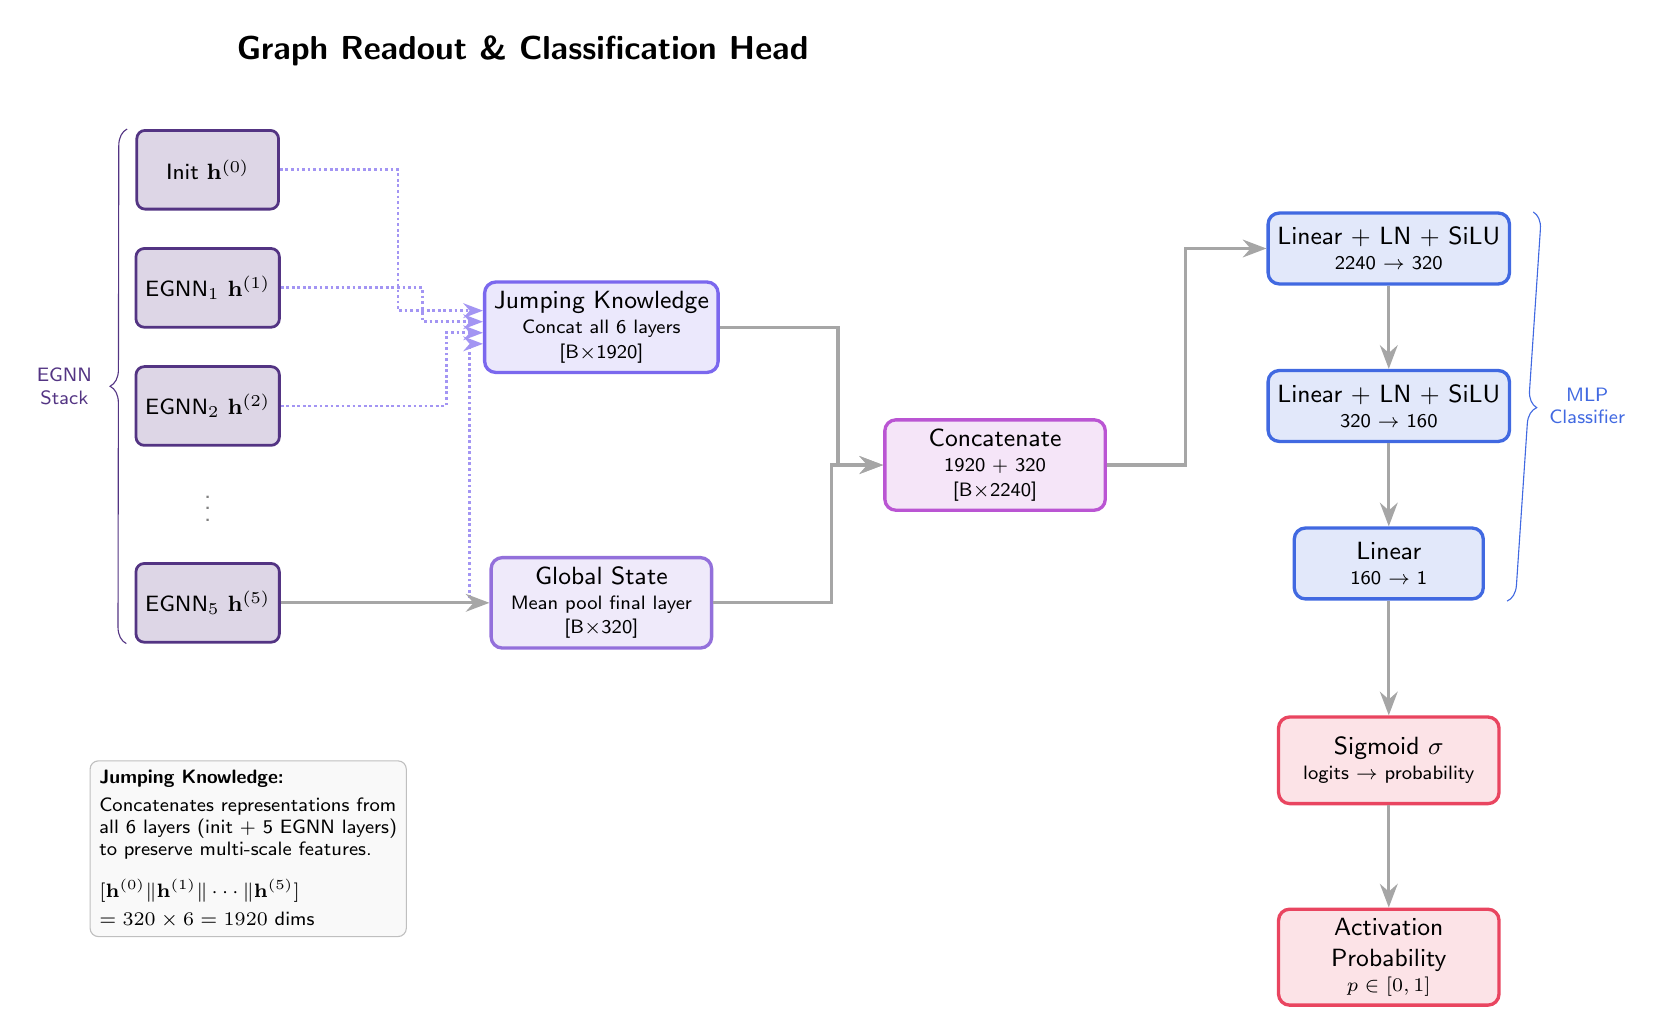
\begin{tikzpicture}[
    % Node styles
    layerblock/.style={
        rectangle,
        rounded corners=3pt,
        draw=egnnCol,
        fill=egnnCol!20,
        line width=1pt,
        font=\sffamily\footnotesize,
        minimum height=1cm,
        minimum width=1.8cm,
        align=center
    },
    block/.style={
        rectangle,
        rounded corners=4pt,
        draw=#1,
        fill=#1!15,
        line width=1.2pt,
        font=\sffamily\small,
        minimum height=1.1cm,
        minimum width=2.8cm,
        align=center
    },
    mlpblock/.style={
        rectangle,
        rounded corners=4pt,
        draw=mlpCol,
        fill=mlpCol!15,
        line width=1.2pt,
        font=\sffamily\small,
        minimum height=0.9cm,
        minimum width=2.4cm,
        align=center
    },
    arrow/.style={
        ->,
        >={Stealth[length=3mm]},
        line width=1.2pt,
        draw=gray!70
    },
    skiparrow/.style={
        ->,
        >={Stealth[length=2.5mm]},
        line width=1pt,
        draw=jkCol!70,
        densely dotted
    },
    brace/.style={
        decorate,
        decoration={brace, amplitude=6pt, raise=3pt, mirror}
    }
]

    % ==== TITLE ====
    \node[font=\sffamily\bfseries\large] at (4, 6.5) {Graph Readout \& Classification Head};
    
    % ==== EGNN LAYERS (LEFT SIDE) ====
    \node[layerblock] (L0) at (0, 5) {Init $\mathbf{h}^{(0)}$};
    \node[layerblock] (L1) at (0, 3.5) {EGNN$_1$ $\mathbf{h}^{(1)}$};
    \node[layerblock] (L2) at (0, 2) {EGNN$_2$ $\mathbf{h}^{(2)}$};
    \node[font=\sffamily, text=gray] at (0, 0.8) {$\vdots$};
    \node[layerblock] (L5) at (0, -0.5) {EGNN$_5$ $\mathbf{h}^{(5)}$};
    
    % Brace for EGNN stack
    \draw[brace, draw=egnnCol] (L0.north west) -- (L5.south west) node[midway, left=12pt, font=\sffamily\scriptsize, text=egnnCol, align=center] {EGNN\\Stack};
    
    % ==== JUMPING KNOWLEDGE ====
    \node[block=jkCol] (jk) at (5, 3) {Jumping Knowledge\\[-2pt]{\scriptsize Concat all 6 layers}\\[-2pt]{\scriptsize [B$\times$1920]}};
    
    % Skip connections to JK - spread out vertically
    \draw[skiparrow] (L0.east) -- ++(1.5, 0) |- ([yshift=6pt]jk.west);
    \draw[skiparrow] (L1.east) -- ++(1.8, 0) |- ([yshift=2pt]jk.west);
    \draw[skiparrow] (L2.east) -- ++(2.1, 0) |- ([yshift=-2pt]jk.west);
    \draw[skiparrow] (L5.east) -- ++(2.4, 0) |- ([yshift=-6pt]jk.west);
    
    % ==== GLOBAL STATE ====
    \node[block=globalCol] (global) at (5, -0.5) {Global State\\[-2pt]{\scriptsize Mean pool final layer}\\[-2pt]{\scriptsize [B$\times$320]}};
    
    % Connection from L5 to Global
    \draw[arrow] (L5.east) -- (global.west);
    
    % ==== CONCATENATION ====
    \node[block=concatCol] (concat) at (10, 1.25) {Concatenate\\[-2pt]{\scriptsize 1920 + 320}\\[-2pt]{\scriptsize [B$\times$2240]}};
    
    % Arrows to concat - go wide to avoid overlap
    \draw[arrow] (jk.east) -- ++(1.5, 0) |- (concat.west);
    \draw[arrow] (global.east) -- ++(1.5, 0) |- (concat.west);
    
    % ==== CLASSIFICATION HEAD ====
    % Positioned to the right with good spacing
    \node[mlpblock] (mlp1) at (15, 4) {Linear + LN + SiLU\\[-2pt]{\scriptsize 2240 $\to$ 320}};
    \node[mlpblock] (mlp2) at (15, 2) {Linear + LN + SiLU\\[-2pt]{\scriptsize 320 $\to$ 160}};
    \node[mlpblock] (mlp3) at (15, 0) {Linear\\[-2pt]{\scriptsize 160 $\to$ 1}};
    
    % Concat to MLP head
    \draw[arrow] (concat.east) -- ++(1, 0) |- (mlp1.west);
    
    % MLP internal connections
    \draw[arrow] (mlp1) -- (mlp2);
    \draw[arrow] (mlp2) -- (mlp3);
    
    % MLP Head brace
    \draw[decorate, decoration={brace, amplitude=6pt, raise=3pt}, draw=mlpCol] 
        ([xshift=5pt]mlp1.north east) -- ([xshift=5pt]mlp3.south east) 
        node[midway, right=10pt, font=\sffamily\scriptsize, text=mlpCol, align=center] {MLP\\Classifier};
    
    % ==== OUTPUT ====
    \node[block=outputCol] (sigmoid) at (15, -2.5) {Sigmoid $\sigma$\\[-2pt]{\scriptsize logits $\to$ probability}};
    \node[block=outputCol] (prob) at (15, -5) {Activation\\Probability\\[-2pt]{\scriptsize $p \in [0,1]$}};
    
    \draw[arrow] (mlp3) -- (sigmoid);
    \draw[arrow] (sigmoid) -- (prob);
    
    % ==== ANNOTATIONS ====
    \node[draw=gray!50, rounded corners=3pt, fill=gray!5, font=\sffamily\scriptsize, align=left, anchor=north west] at (-1.5, -2.5) {
        \textbf{Jumping Knowledge:}\\[2pt]
        Concatenates representations from\\
        all 6 layers (init + 5 EGNN layers)\\
        to preserve multi-scale features.\\[6pt]
        $[\mathbf{h}^{(0)} \| \mathbf{h}^{(1)} \| \cdots \| \mathbf{h}^{(5)}]$\\[2pt]
        $= 320 \times 6 = 1920$ dims
    };

\end{tikzpicture}
\end{document}